%=============================================================================%
% Author : Alejandro P�rez Ruiz                                               %
% Author : Pablo S�nchez Barreiro                                             %
% Version: 1.1, 10/06/2011                                                    %
% Master Thesis: Background, master file                                      %
%=============================================================================%

\chapterheader{Antecedentes}{Antecedentes}
\label{chap:background}

Este cap�tulo proporciona una muy breve introducci�n a las diferentes t�cnicas y tecnolog�as que se usar�n a lo largo de este proyecto y que se entiende que no tienen por qu� ser conocidas por el lector. M�s concretamente, ofrece una visi�n general de las l�neas de productos software, el desarrollo de software orientado a caracter�sticas y las clases parciales de C\#. Recordemos que el objetivo de este proyecto es implementar una l�nea de productos usando clases parciales de C\# como mecanismo para encapsular y componer caracter�sticas.

\chaptertoc

\section{L�neas de Productos Software}

%%==================================================================%%
%% Author : Abascal Fern�ndez, Patricia                             %%
%%          S�nchez Barreiro, Pablo                                 %%
%% Version: 1.3, 18/06/2013                                         %%
%%                                                                  %%
%% Memoria del Proyecto Fin de Carrera                              %%
%% Background/Software Product Lines                                %%
%===================================================================%%

El objetivo de una \emph{l�nea de producto software}~\citep{pohl:2010,kakola:2006} es crear una infraestructura adecuada a partir de la cual se puedan derivar, de forma tan autom�tica como sea posible, producto concretos pertenecientes a una familia de producto software. Una familia de producto software es un conjunto de aplicaciones software similares, lo que implica que comparten una serie de caracter�sticas comunes, pero que tambi�n presentan variaciones entre ellos.

Un ejemplo cl�sico de familia de producto software es el producto Parten�n, para software bancario, comentado en la introducci�n a este documento (ver Secci�n~\ref{sec:intr:introduction}). Dicho producto representa una familia de productos destinados a la gesti�n bancaria. Parten�n en s� no puede ser desplegado como una aplicaci�n, sino que necesita ser configurado de acuerdo a una serie de caracter�sticas concretas demandadas por cada cliente que require una instalaci�n de Parten�n.

La idea de una l�nea de producto software es proporcionar una forma autom�tica y sistem�tica de construir productos concretos dentro de una familia de producto software mediante la simple especificaci�n de qu� caracter�sticas deseamos incluir dentro de dicho producto. Esto representa una alternativa al enfoque tradicional de desarrollo software, el cual se basaba simplemente en seleccionar el producto m�s parecido, dentro de la familia, al que queremos construir y adaptarlo manualmente.

El proceso de creaci�n de l�neas de producto software se estructura dos fases: (1) \emph{Ingenier�a del Dominio} (en ingl�s,  \emph{Domain Engineering}); y (2) \emph{Ingenier�a de Aplicaci�n} (en ingl�s, \emph{Application Engineering}) (ver Figura~\ref{back:fig:domainAplicEng}). La \emph{Ingenier�a del Dominio} tiene como objetivo la creaci�n de la infraestructura o arquitectura de referencia de la l�nea de productos software. Esta arquitectura de referencia debe permitir la r�pida, o incluso autom�tica, construcci�n de sistemas software espec�ficos pertenecientes a la familia de productos software. La \emph{Ingenier�a de Aplicaci�n} utiliza la infraestructura creada anteriormente para crear aplicaciones espec�ficas adaptadas a las necesidades de cada usuario en concreto.

\begin{figure}[!tb]
  \centering
  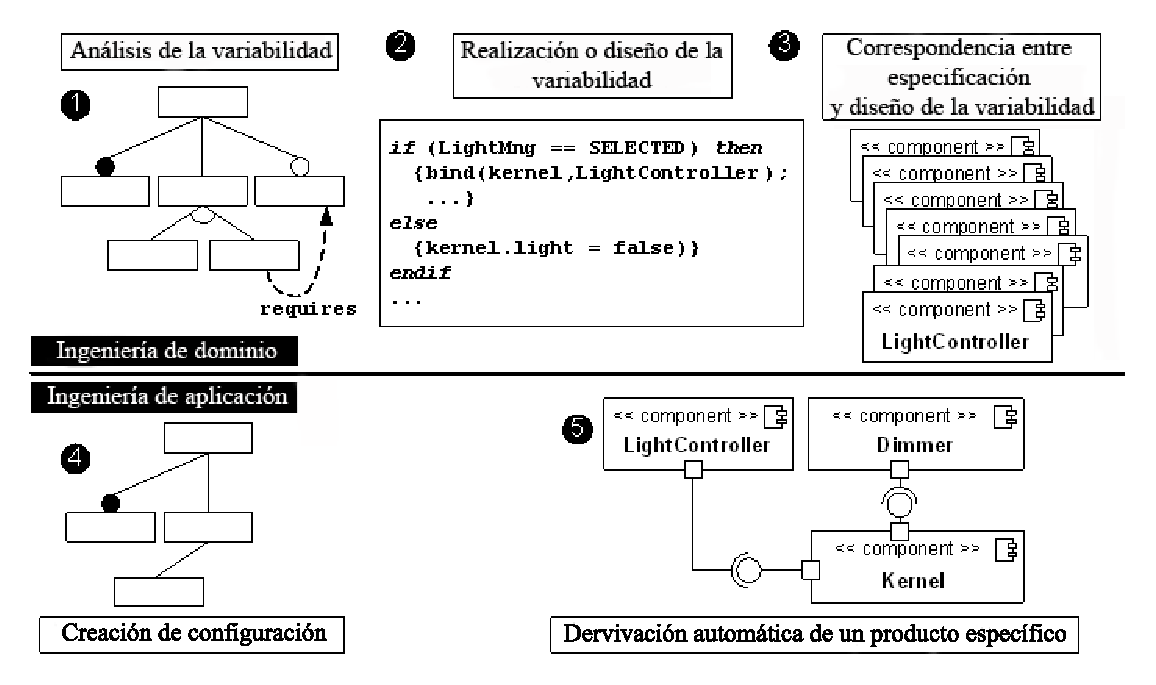
\includegraphics[width=.95\linewidth]{background/images/domainAplicationEngineering.eps} \\
  \caption{Proceso de Desarrollo de una l�nea de producto software}
  \label{back:fig:domainAplicEng}
\end{figure}

En la fase de Ingenier�a del Dominio, el primer paso a realizar es un an�lisis de qu� caracter�sticas de la familia de producto son variables y por qu� son variables. Esta parte es la que se conoce como \emph{An�lisis o Especificaci�n de la Variabilidad} (Figura~\ref{back:fig:domainAplicEng}, etiqueta 1).

A continuaci�n, se ha de dise�ar una arquitectura de referencia para la familia de producto software que permita soportar dicha variabilidad. Esta actividad se conoce como \emph{Realizaci�n o Dise�o de la Variabilidad} (Figura~\ref{back:fig:domainAplicEng}, etiqueta 2).

El siguiente paso es establecer una serie de reglas que especifiquen c�mo hay que instanciar o configurar la arquitectura previamente creada de acuerdo con las caracter�sticas seleccionadas por cada cliente. Esta fase es la que se conoce como \emph{Correspondencia entre Especificaci�n y Dise�o de la Variabilidad} (Figura~\ref{back:fig:domainAplicEng}, etiqueta 3).

Tras completar la fase de Ingenier�a del Dominio, disponemos de una especie de l�nea de montaje, la cual podemos utilizar para construir productos concretos de forma m�s o menos automatizada.

En la fase de Ingenier�a de Aplicaci�n, se crean productos concretos utilizando la infraestructura previamente creada. Para ello, el primer paso es crear una \emph{configuraci�n}, que no es m�s que una selecci�n de caracter�sticas que un usuario desea incluir en su producto concereto (Figura~\ref{back:fig:domainAplicEng}, etiqueta 4).

En el caso ideal, usando esta configuraci�n, se debe poder ejecutar las reglas de correspondencia entre especificaci�n y dise�o de la variabilidad para que la arquitectura creada en la fase de Ingenier�a del Dominio se adapte autom�ticamente; generando un producto concreto espec�fico acorde a las necesidades concretas del usuario (Figura~\ref{back:fig:domainAplicEng}, etiqueta 5). En el caso no ideal, dichas reglas de correspondencia deber�n ejecutarse a mano, lo cual suele ser un proceso tedioso, largo, repetitivo y propenso a errores.

La siguiente secci�n describe el paradigma de desarrollo software orientada a caracter�sticas, el cual est� �ntimamente ligado al dise�o e implementaci�n de l�neas de productos software.



\section{Ejemplo de LPS: El Problema de las Expresiones}

%=============================================================================%
% Author : Alejandro P�rez Ruiz                                               %
% Author : Pablo S�nchez Barreiro                                             %
% Version: 1.1, 10/06/2011                                                    %
% Master Thesis: Background/Expression Problem                                %
%=============================================================================%

El \emph{problema de las expresiones} es un problema t�pico dentro del mundo del dise�o software~\cite{cook:1990,togersen:2004} y que es muy frecuentemente utilizado para ilustrar el funcionamiento de las diferentes t�cnicas y tecnolog�as relacionadas con las l�neas de productos software~\cite{lopezHerrejon:2004}. El objetivo del problema de las expresiones es dise�ar una familia de productos software que, para la gram�tica de la Figura~\ref{back:fig:gramExpr}, soporte las siguientes operaciones:

\begin{description}
	\item[Print:] Debe mostrar por consola la expresi�n en el formato infijo, prefijo o posfijo.
	\item[Eval:] Debe evaluar la expresi�n y retornar su resultado.
	\item[ShortEval:] debe evaluar la expresi�n realizando las operaciones \emph{cortocircuitadas}. Es decir, tan pronto como el valor de un operando determine el resultado de la expresi�n, se deber� parar la evaluaci�n del resto de los operandos. Por ejemplo, en una multiplicaci�n, si el primer operando es 0, se retornar� el valor 0 directamente, sin evaluar el segundo operando.
\end{description}

No todas las operaciones tienen que aparecer en todos los productos, por lo que deber�a ser posible construir productos concretos que careciesen de alguna de ellas. Por tanto, se identifican dos conjuntos diferenciados de caracter�sticas: (1) las operaciones \imp{\{Print, Eval, ShortEval\}} que se pueden realizar sobre la gram�tica; y (2) si la notaci�n de los operadores es infija, prefija o postfija.

\begin{figure}
\begin{center}
\begin{footnotesize}
\begin{verbatim}
Exp :: = Integer | AddInfix | MultInfix | AddPostfix | MulltPostfix |
				 AddPrefix | MultPrefix
Integer     :: <positive-negative integers>
AddInfix    ::= Exp "+" Exp
MultInfix   ::= Exp "*" Exp
AddPostfix  ::= Exp Exp "+"
MultPostfix ::= Exp Exp "*"
AddPrefix   ::= "+" Exp Exp
MultPrefix  ::= "*" Exp Exp
\end{verbatim}
\end{footnotesize}
\end{center}
\caption{Gram�tica del lenguaje de expresiones}
\label{back:fig:gramExpr}
\end{figure}

La siguiente secci�n describe c�mo usando �rboles de caracter�sticas podemos especificar la variabilidad existente en esta familia de productos software.



\section{�rboles de Caracter�sticas}
\label{back:sec:feature}

%=============================================================================%
% Author : Alejandro P�rez Ruiz                                               %
% Author : Pablo S�nchez Barreiro                                             %
% Version: 1.1, 10/06/2011                                                    %
% Master Thesis: Background/Feature Model                                     %
%=============================================================================%

Un �rbol de caracter�sticas~\cite{kang:1990,benavides:2010} es un �rbol and-or que se usa para especificar que elementos de una familia de productos (software)
son comunes a toda la familia de productos software, cuales son variables y por qu� dichos elementos son variables, por ejemplo, porque sean opcionales o alternativos entre s�.

La Figura~\ref{back:fig:featureModel} muestra un �rbol de caracter�sticas para una l�nea de productos software para el problema de las expresiones descrito en la secci�n anterior.  


Identificamos en este problema dos conjuntos diferenciados de caracter
��sticas: (1) las operaciones {Print, Eval, ShortEval} que se pueden realizar
sobre la gram�atica; y (2) si los operadores son infijos, prefijos o postfijos. Por
tanto, tenemos 6 caracter��sticas posibles para nuestros productos (operadores
infijos, prefijos o postfijos, m�as {Print, Eval, ShortEval} como operaciones
opcionales para la gram�atica). Tras haber descompuesto el problema en sus
diferentes caracter��sticas se ha modelado un diagrama de caracter��sticas representado
en la figura 2.5 con las peculiaridades anteriormente descritas.





%%=========================================================================%%
%% NOTA(Pablo): Esto se explica sobre la misma figura, eliminalo           %%                      %%=========================================================================%%
%%
%% Las relaciones entre las caracter�sticas padres y las caracter�sticas hijas
%% pueden ser clasificadas como:
%% \begin{enumerate}
%%    \item \emph{Obligatoria}: La caracter�stica hija es obligatoria.
%%    \item \emph{Opcional}: La caracter�stica hija es opcional.
%%    \item \emph{Simple}: La caracter�stica hija tendr� cardinalidad
%%            \emph{<m..n>}
%%    \item \emph{Grupo Or}: Al menos una de las caracter�sticas hijas debe ser
%%            seleccionada.
%%    \item \emph{Grupo Xor}: S�lo una de las caracter�sticas hijas debe ser
%%            seleccionada
%%    \item \emph{Grupo-Simple}: El n�mero de caracter�sticas seleccionadas del
%%            grupo vendr� dado por su cardinalidad.
%% \end{enumerate}
%%
%% Para representar visualmente las relaciones descritas anteriormente se
%% utiliza la notaci�n que se puede observar en la figura \ref{}.
%% \begin{figure}[!tb]
%%  \centering
%% 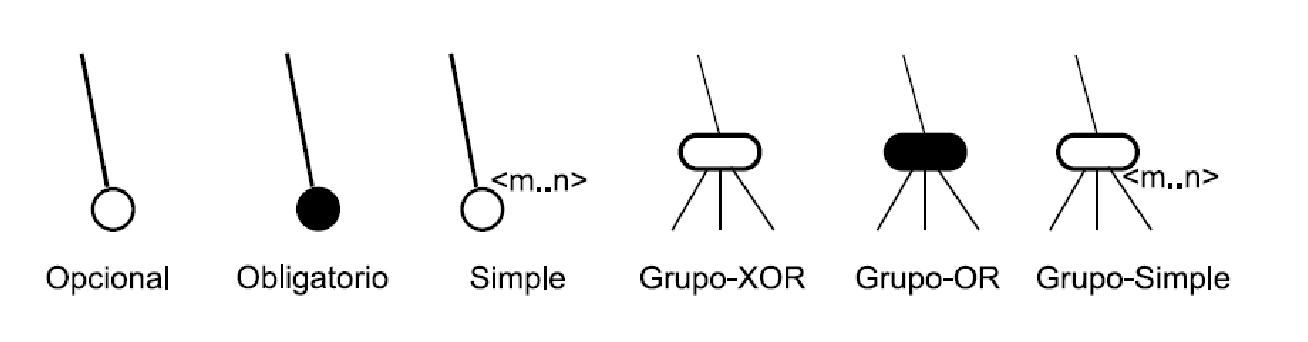
\includegraphics[width=.65\linewidth]{background/images/notFeatureDiagram.eps} %% \\
%%  \caption{Notaciones utilizadas en los diagramas de caracter�sticas}
%%  \label{back:fig:fesatureModel}
%% \end{figure}
%%=========================================================================%%

Adem�s de las relaciones las caracter�sticas pueden tener restricciones, com�nmente las m�s utilizadas son requiere(si selecciona la caracter�stica A implica seleccionar la caracter�stica B) y excluye (si se selecciona la caracter�stica A la caracter�stica B debe ser excluida), pero puede ser utilizada cualquier f�rmula l�gica que describa una restricci�n.

El objetivo de este tipo de diagramas a parte de la propia representaci�n y facilidad para visualizar las diferentes caracter�sticas, es la posibilidad de utilizar las transformaciones de modelos para conseguir realizar configuraciones que satisfagan las restricciones\cite{czarnecki:2004}.

A modo de ejemplo se incluye en la figura \ref{back:fig:featurEShop} el diagrama de caracter�sticas que muestra un sistema configurable para una tienda online.

\begin{figure}[!tb]
  \centering 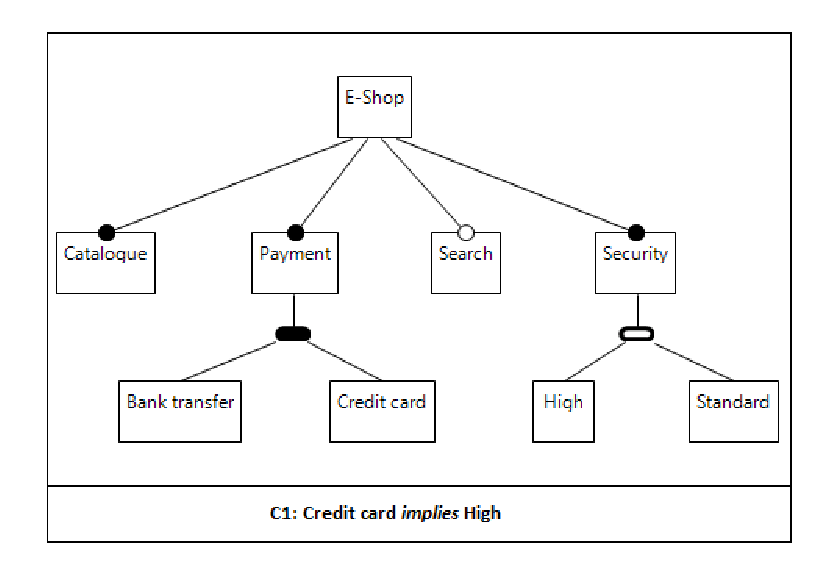
\includegraphics[width=.85\linewidth]{background/images/featureModelEshop.eps} \\
  \caption{Diagrama de caracter�sticas para una \emph{e-shop}}
  \label{back:fig:featurEShop}
\end{figure}

Cuando se modelan l�neas de productos software a trav�s de los diagramas de caracter�sticas,y se pretende generar el c�digo necesario para crear una familia de productos software, los lenguajes de programaci�n orientados a objetos resultan muchas veces insuficientes. Con objeto de paliar estas deficiencias, en los �ltimos a�os han ido surgiendo unos nuevos tipos de lenguajes denominados \emph{orientados a caracter�sticas}. La siguiente secci�n introduce la programaci�n orientada a caracter�sticas para a continuaci�n explicar sus ventajas con respecto a las t�cnicas tradicionales orientadas a objetos.


\section{Programaci�n Orientada a Caracter�sticas}

%=========================================================================%
% Author : Alejandro P�rez Ruiz                                           %
% Author : Pablo S�nchez Barreiro                                         %
% Version: 1.1, 10/06/2011                                                %
% Master Thesis: Background/Feature Oriented Programming                  %
%=========================================================================%

La programaci�n orientada a caracter�sticas~\cite{prehofer:2001} surge como respuesta a las limitaciones que el dise�o y la programaci�n orientada a objetos posee en relaci�n a la implementaci�n de las l�nea de productos software. Por tanto, antes de describir en qu� consiste la programaci�n orientada a caracter�sticas, comentaremos qu� propiedades ser�an deseables encontrar en un lenguaje para la implementaci�n de l�neas de productos software y analizaremos c�mo satisfacer las t�cnicas de desarrollo software orientado a objetos dichas propiedades, comentando sus principales limitaciones.

\subsection{Propiedades deseables de un lenguaje de programaci�n para la implementaci�n de l�neas de productos software}
\label{back:subsec:propiedades}

%=========================================================================%
% Author : Alejandro P�rez Ruiz                                           %
% Author : Pablo S�nchez Barreiro                                         %
% Version: 1.1, 10/06/2011                                                %
% Master Thesis: Background/FeatureOrientedChallenge                      %
%=========================================================================%

Siguiendo los estudios y trabajos realizados por \cite{lopez:2005,chul:2002,aracic:2006,chae:2009,elio:2010} se  identifican  en esta secci�n una serie de elementos que ser�a deseable encontrar en un lenguaje orientado a caracter�sticas.

\paragraph{Extensi�n a trav�s de la adici�n y la sustituci�n:}

Una caracter�stica se considera normalmente un incremento en la funcionalidad de un sistema software~\cite{batory:2004}. Las extensiones pueden ser tanto por adici�n de nueva funcionalidad (e.g., evaluaci�n de expresiones), como por sustituci�n o sobreescritura de funcionalidades ya existentes (e.g., evaluaci�n con cortocircuito). Por lo tanto, para la implementaci�n de una l�nea de productos software ser�a deseable encontrar en un lenguaje de programaci�n mecanismos que permitiesen extender y sobreescribir las funcionalidades ya existentes.

\paragraph{Encapsulamiento de caracter�sticas:}

Todas las extensiones pertenecientes a una caracter�stica concreta se deber�an poder a�adir o eliminar de forma at�mica de un determinado producto. Es decir, o se a�aden todas las extensiones a un producto, o no se a�ade ninguna. Por lo tanto, un lenguaje adecuado para la implementaci�n de l�neas de productos software deber�a proporcionar mecanismos para agrupar y encapsular los elementos pertenecientes a una misma caracter�stica en un �nico modulo software cuya composici�n fuese lo m�s f�cil posible. Estos m�dulos deber�an adem�s permitir su  desarrollo y compilaci�n independiente.

\paragraph{Composici�n a nivel de caracter�stica:}

En una l�nea de productos software, los productos software concretos acordes a las necesidades particulares de cada cliente se obtienen mediante la selecci�n y composici�n de las caracter�sticas deseadas por cada cliente. Por lo tanto, ser�a deseable que un lenguaje de programaci�n para la implementaci�n de l�neas de productos software proporcionase facilidades para especificar dicha composici�n. Tal composici�n deber�a adem�s realizarse a nivel de caracter�stica, indicando que caracter�sticas deseamos componer, en lugar de tener que especificar que elementos individuales dentro de cada caracter�stica debemos componer.

\paragraph{An�lisis y gesti�n de la correcci�n de la composici�n:}

Cuando se desea componer un producto concreto dentro de una l�nea de productos software, no todas las combinaciones de caracter�sticas dan lugar a productos v�lidos. Por lo tanto, ser�a deseable que un lenguaje utilizado para la implementaci�n de l�neas de productos software pudiese detectar composiciones err�neas, alertando a los desarrolladores de los posibles fallos. Adem�s, en la medida de lo posible, dichos fallos deber�an solventarse, siempre que fuese posible, de forma autom�tica mediante la gesti�n de las restricciones y dependencias entre caracter�sticas por parte del propio lenguaje.

La siguiente subsecci�n analiza como las t�cnicas orientadas a objetos satisfacen estas caracter�sticas. 

\subsection{Limitaciones de la orientaci�n a objetos respecto a la implementaci�n de l�neas de productos software}
\label{back:sub:limitacionesOO}

\input{background/OOshortcomings.tex}

\subsection{Lenguajes de programaci�n orientados a caracter�sticas}
\label{back:subsec:foLanguages}

Los lenguajes orientados a caracter�sticas~\cite{prehofer:2001} tienen como objetivo encapsular conjuntos coherentes de funcionalidad de un sistema software en m�dulos independientes y f�cilmente componibles de forma que se incremente la capacidad de reutilizaci�n y extensi�n de estos m�dulos. Dichos m�dulos reciben el nombre de \emph{caracter�stica}. Una caracter�stica se suele definir como un incremento de la funcionalidad de un sistema~\cite{batory:2004}.

%%===============================================================================================================%%
%% NOTA(Pablo): Tal como se ha reorganizado esta secci�n, esto ha quedado ya bastante claro                      %%
%%===============================================================================================================%%
%%
%% Los lenguajes orientados a caracter�sticas son especialmente �tiles en el contexto de las l�neas de productos
%% software, ya que nos permiten encapsular en m�dulos bien definidos las diferentes caracter�sticas, tanto comunes %% como variables, que pueden aparecer en cada uno de los productos software pertenecientes a una misma familia. Los %% lenguajes orientados a caracter�sticas tratan de facilitar adem�s la composici�n de dichos m�dulos, contribuyendo %% as� a que productos espec�ficos dentro de una familia puedan ser creados mediante la simple composici�n o
%% ensamblado de m�dulos software relativamente independientes.
%%
%%===============================================================================================================%%

%%============================================================================%%
%% NOTA(Pablo): Con la nueva reestructuraci�n de la secci�n, esta             %%
%%     argumentaci�n sobra                                                    %%
%%============================================================================%%
% Por ejemplo, a la hora de crear un tipo abstracto de datos pila, podemos
% considerar diferentes variaciones:
% \begin{description}
%     \item[B�sicas:] Toda pila, para ser considerada pila, debe soportar las
%            operaciones \imp{apilar} y \imp{desapilar}.
%     \item[Contador:] A�ade un contador para conocer el tama�o de la pila.
%     \item[Bloqueo:] Permite bloquear la pila para evitar modificaciones en su
%            estado.
%     \item[Deshacer:] Agrega la funcionalidad de restaurar el estado de la pila %            antes del �ltimo acceso a la misma.
% \end{description}
%
% El objetivo de la programaci�n orientada a caracter�sticas ser�a encapsular
% cada una de las cuatro funcionalidades anteriores en m�dulos independientes y
% f�cilmente componibles. De esta forma, se podr�an obtener diferentes productos % mediante la simple composici�n de conjuntos diferentes de caracter�sticas. Por % ejemplo, un determinado usuario podr�a estar interesado en una pila con
% contador, por lo que compondr�a estas dos caracter�sticas y descartar�a las
% dem�s. Otro usuario podr�a encontrar m�s adecuada una pila con bloqueo y
% deshacer, por lo que compondr�a estas tres caracter�sticas y dejar�a fuera la
% correspondiente al contador.
%
% Por lo tanto, un lenguaje orientado a caracter�sticas nos debe permitir
% descomponer f�cilmente un programa en caracter�sticas, las cuales deber�an
% encapsularse en m�dulos bien definidos y tan independientes como sea posible.
% A la hora de crear productos concretos, dichos m�dulos se compondr�an de
% acuerdo a las necesidades de los usuarios.
%%============================================================================%%

%%=====================================================================================================%%
%% NOTA(Pablo): Esto tambi�n me parece redundante ahora                                                %%
%%=====================================================================================================%%
%%
%% \subsubsection{Conclusiones}
%%
%% Tras analizar el problema con un lenguaje orientado a objetos como es C\# se podr�a determinar que
%% ser�a deseable %% encontrar un nuevo paradigma de  programaci�n, orientado a caracter�sticas, donde
%% se pudiesen obtener f�cilmente diferentes versiones de una misma aplicaci�n mediante la simple
%% composici�n de caracter�sticas. Obviamente no todas las combinaciones de caracter�sticas ser�an
%% v�lidas, por ejemplo para una caracter�stica de una aplicaci�n para un hogar inteligente que se
%% encargue de realizar un uso eficiente del consumo de energ�a a trav�s del control de las perdidas
%% por ventanas abiertas, necesitar� que las caracter�sticas relacionadas con la calefacci�n y las
%% ventanas est�n seleccionadas. Por tanto, un lenguaje orientado a caracter�sticas deber�a asegurarse
%% de que el resultado de la composici�n de un conjunto de caracter�sticas da lugar a aplicaciones
%% v�lidas y consistentes.
%%
%%=====================================================================================================%%

%%=====================================================================================================%%
%% NOTA(Pablo): Esto tambi�n me parece redundante ahora                                                %%
%%=====================================================================================================%%
%%
%% \subsection{Ventajas de los lenguajes orientados a caracter�sticas}
%%
%% Los lenguajes orientados a caracter�sticas nos otorgan una mayor flexibilidad, ya que nos permiten
%% que clases individuales puedan ser compuestas por un conjunto de caracter�sticas, por tanto son
%% especialmente recomendados %% para utilizarlos con las l�neas de producci�n software.
%%
%%=====================================================================================================%%

Para estudiar las ventajas de los lenguajes orientados a caracter�sticas nos basaremos en las facilidades proporcionadas por CaesarJ~\cite{aracic:2006}, aunque ilustraremos los ejemplos con diagramas UML. Para mostrar las ventajas de dicho lenguaje se usar� el ya comentado problema de las expresiones\footnote{Dicha implementaci�n se proporciona en el soporte �ptico adjunto a esta memoria.}. CaesarJ es un lenguaje de programaci�n orientado a caracter�sticas basado en Java. Para ello trabaja con el concepto de \emph{familia de clases}. Una \emph{familia de clases} es una unidad de encapsulamiento que sirve para agrupar clases relacionadas. Las familias de clases reciben un tratamiento similar al de las clases, soportando relaciones de herencia entre ellas.

Adem�s, CaesarJ tambi�n introduce el concepto de \emph{clases virtuales}. Una clase virtual es una clase perteneciente a una familia de clases y que es susceptible de ser heredada y sobreescrita por familias de clases que hereden de la familia de clases que contiene dicha clase virtual. La Figura~\ref{} ilustra esta situaci�n. Las familias de clases se representan mediante paquetes UML, y herencia entre clases, mediante relaciones \emph{merge}. Cuando una familia de clases hereda de otra, hereda impl�citamente todas sus clases virtuales. Si la primera contiene clases virtuales con el mismo nombre que la familia de clases que hereda, entonces la clase virtual de la familia de clases hija hereda de la clase virtual con el mismo nombre de la familia de clases padre. Por ejemplo, en la Figura~\ref{}, la clase \imp{Mult} de la familia de clases \imp{Eval} heredar�a impl�citamente de la clase \imp{Mult} de la familia de clases \imp{Basic}. En cada familia de clases hija, se pueden a�adir por tanto nuevos atributos y m�todos a las clases virtuales de las familias de clases padre. Adem�s, gracias al avanzado sistema de tipos de CaesarJ, se pueden a�adir nuevas relaciones de herencia.

%%=====================================================================================================%%
%% NOTA(Pablo): Aqu� va haciendo falta un ejemplo, y mejor que el que est� en la Figura 1.8. Haz un
%%              ejemplo como el del art�culo del FOSD 2010, que se vean las clases dentro de los
%%              paquetes para al menos dos caracter�sticas, por ejemplo expression y eval
%%=====================================================================================================%%

Adem�s, las referencias entre clases se actualizan autom�ticamente. Por ejemplo, en el caso de la Figura~\ref{}, aunque no se haga expl�citamente, cualquier referencia a una clase del tipo \imp{Expression} dentro de la familia de clases \imp{Eval} se referir� a la clase virtual \imp{Expression} de la familia de clases \imp{Eval} y no a la clase virtual de mismo nombre de la familia de clases \imp{Basic}. De esta forma, las referencias est�n siempre actualizadas a su versi�n m�s extendida.

Para implementar una l�nea de productos software, cada caracter�stica se considera como una familia de clases.
Dentro de cada familia de clases, cada caracter�stica se dise�a usando las t�cnicas tradicionales de la orientaci�n a objetos, tal como se muestra en la Figura~\ref{}.

%%======================================================================================================%%
%% NOTA(Pablo): Esto ahora quedar�a redundante                                                          %%
%%======================================================================================================%%
%%
%% La figura~\ref{back:fig:caesarJExpressions} muestra que por cada operaci�n, tenemos una familia de
%% clases, siendo la familia de clases que encapsula a todas las dem�s, la denominada \imp{Expressions}.
%% �sta tiene la estructura de clases representado en la figura \ref{back:fig:expr}, y cada familia de
%% clases lo que hace es redefinir las clases virtuales de \imp{Expressions} con las operaciones
%% necesarias en cada caso.
%%
%%======================================================================================================%%

\begin{figure}[ht!]
  % Requires \usepackage{graphicx}
  \centering 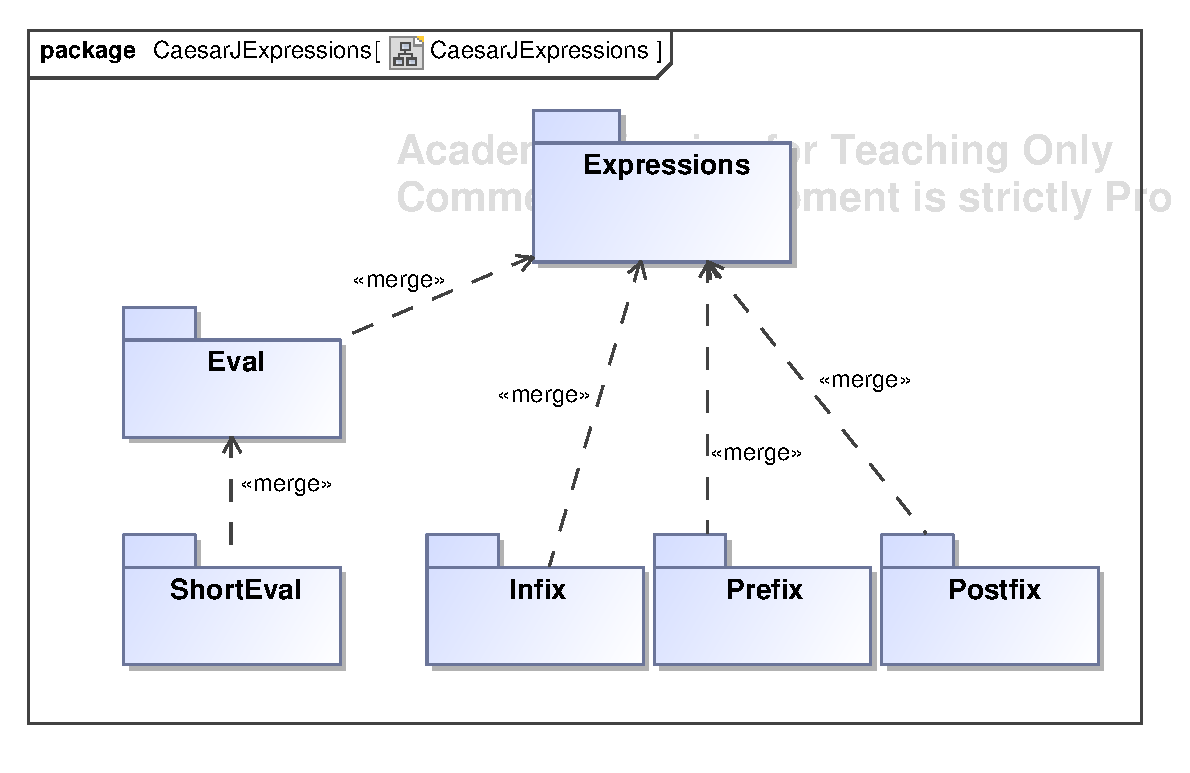
\includegraphics[width=.60\linewidth]{background/images/CaesarJExpressions.eps} \\
  \caption{Dise�o para resolver el problema de las expresiones con CaesarJ}
  \label{back:fig:caesarJExpressions}
\end{figure}
\begin{figure}[ht!]
\begin{center}
\begin{footnotesize}
\begin{verbatim}
00 import eval.Eval;
01 import printPostfix.PrintPostfix;
02 import printInfix.PrintInfix;
03 import printPrefix.PrintPrefix;
04 public cclass EvalInfix extends PrintPrefix & Eval {}
\end{verbatim}
\end{footnotesize}
\end{center}
\caption{Configuraci�n que incluye las operaciones de evaluar e imprimir en formato infijo con CaesarJ}
\label{back:fig:codCaesarJ}
\end{figure}

Para realizar una configuraci�n, es decir, para crear un producto concreto por composici�n de caracter�sticas, simplemente hay que crear una nueva familia de clases que herede de las familias de clases que correspondan a las caracter�sticas seleccionadas. La figura \ref{back:fig:codCaesarJ} muestra como se crear�a un producto nuevo mediante la composici�n de las caracter�sticas \imp{Eval} e \imp{Infix}.

%%======================================================================================================%%
%% NOTA(Pablo): Queda raro haber estado mostrando diagramas hasta ahora y luego poner c�digo, as� que   %%
%%              haz un diagrama de una configuraci�n y quita el c�digo                                  %%
%%======================================================================================================%%

%%======================================================================================================%%
%% NOTA(Pablo): Completa este an�lisis                                                                  %%
%%======================================================================================================%%

A continuaci�n analizamos como la programaci�n orientada a caracter�sticas satisface las propiedades que
debe poseer un lenguaje de programaci�n para la implementaci�n de las l�neas de productos software:

\paragraph{Extensi�n a trav�s de la adici�n y la sustituci�n:}

\paragraph{Encapsulamiento de caracter�sticas:}

\paragraph{Composici�n a nivel de caracter�stica:}

\paragraph{An�lisis y gesti�n de la correcci�n de la composici�n:}

%%======================================================================================================%%
%% NOTA(Pablo): Aqu� d� que todo esto est� muy bonito, pero que hay que cambiar el lenguaje de          %%
%%              programaci�n y que las empresas no quieren por los problemas que se comentan en la      %%
%%              introducci�n y que por tanto lo queremos hacer con C\#, bla bla bla  y enlaza con       %%
%%              la siguiente secci�n                                                                    %%
%%======================================================================================================%%


\section{Clases Parciales C\#}

%=========================================================================%
% Author : Alejandro P�rez Ruiz                                           %
% Author : Pablo S�nchez Barreiro                                         %
% Version: 1.1, 10/06/2011                                                %
% Master Thesis: Background/PartialClasses                                %
%=========================================================================%

Las clases parciales C\# \cite{albahari:2010} permiten dividir la implementaci�n de una clase en varios archivos de c�digo fuente. Cada fragmento representa una parte de la funcionalidad global de la clase. Todos estos fragmentos se combinan en tiempo de compilaci�n para crear una �nica clase, la cual contiene toda la funcionalidad especificada en las clases parciales. Por lo tanto, las clases parciales C\# parecen un mecanismo adecuado para implementar caracter�sticas, tal como ha sido identificado por diversos autores~\cite{laguna:2007,laguna:2010}, dado que cada incremento en funcionalidad perteneciente a una caracter�stica se podr�a encapsular en una clase parcial separada.

%%==============================================================================================================%%
%% NOTA(Pablo): Poner un ejemplo peque�o aqu� con dos clases parciales relativas al problema de las expresiones %%
%%==============================================================================================================%%

%%=============================================================================================================%%
%% NOTA(Pablo): Esto no me cuadra muy bien aqu�, as� que lo borro                                              %%
%%=============================================================================================================%%
%%
%% Para poder ser compiladas y agrupadas en una sola clase, todas las clases parciales deben pertenecer al
%% mismo espacio de nombres, poseer la misma visibilidad y deben ser declaradas con la palabra clave
%% \imp{partial}. En C\#, un espacio de nombre se emplea simplemente para agrupar clases relacionadas y evitar
%% conflictos de nombres.
%%
%%=============================================================================================================%%


Para especificar los archivos C\# que deben ser incluidos en una unidad de compilaci�n se emplea un documento XML como el de la Figura~\ref{back:fig:partialClass}. Por lo tanto, es posible incluir y excluir f�cilmente la funcionalidad encapsulada dentro de una clase parcial simplemente a�adiendo o eliminando dicha clase parcial de este fichero XML. Por tanto, la composici�n de caracter�sticas tambi�n parece factible mediante la manipulaci�n de este fichero XML.

\begin{figure}[!h]
\begin{center}
\begin{footnotesize}
\begin{verbatim}
01    <itemgroup>
02    <!--Eval-->
03    <Compile Include="Eval\Add.cs" />
04    <Compile Include="Eval\IExpressionsEval.cs" />
05    <Compile Include="Eval\IExpressions.cs" />
06    <Compile Include="Eval\Integer.cs" />
07    <Compile Include="Eval\Mult.cs" />
08    <!--Infix-->
09    <!--<Compile Include="Infix\Add.cs" />
10    <Compile Include="Infix\IExpressionInfix.cs" />
11    <Compile Include="Infix\IExpressions.cs" />
12    <Compile Include="Infix\Integer.cs" />
13    <Compile Include="Infix\Mult.cs" />-->
14    ...
15    </itemgroup>
16    </Project>
\end{verbatim}
\end{footnotesize}
\end{center}
\caption{Archivo XML que guarda la informaci�n para la compilaci�n en Visual Studio}
\label{back:fig:partialClass}
\end{figure}

%%=============================================================================================================%%
%% NOTA(Pablo): Esto no me cuadra muy bien aqu�, as� que lo borro                                              %%
%%=============================================================================================================%%
%% Para ilustrar lo dicho anteriormente, se ha vuelto a utilizar el problema de las expresiones implement�ndolo
%% con clases parciales. La figura \ref{back:fig:partialClass} muestra como hemos excluido de la compilaci�n la
%% caracter�stica que representa la operaci�n de imprimir una expresi�n en formato infijo.
%% Este mecanismo de clases parciales permite a�adir o compartir funcionalidad entre un conjunto de clases que
%% no precisan estar relacionadas mediante ning�n tipo de relaci�n jer�rquica, tal como ocurre con la herencia.



\section{Sumario}

Durante este cap�tulo se han descrito los conceptos necesarios para entender la motivaci�n de este proyecto. Se ha descrito qu� es una l�nea de productos software, las t�cnicas utilizadas para su desarrollo, las limitaciones de la orientaci�n a objetos para su implementaci�n y las ventajas de los lenguajes orientados a caracter�sticas. No obstante, tal como se ha comentado, en muchas situaciones o los lenguajes de programaci�n orientados a caracter�sticas no est�n siempre lo suficientemente maduros como para ser transferidos a la industria, o las empresas no pueden permitirse el coste asociado a cambiar su lenguaje de programaci�n habitual. Por tanto, una posible soluci�n, ser�a intentar implementar l�neas de productos software usando las construcciones proporcionadas por un lenguaje de programaci�n de amplia difusi�n, tal como C\#. Por dicho motivo, en las siguientes secciones implementaremos una l�nea de productos software para hogares inteligentes usando las clases parciales de C\#. El siguiente cap�tulo describe la planificaci�n general seguida para la realizaci�n de este proyecto.

